\subsection{Quality Metrics of an Individual Layer as an HCIZ Integral}
\label{sxn:matgen_quality_hciz}

In this subsection, we describe how to generalize the (Thermal) average over the Students $\THRMAVG{\cdots}$ to an 
integral over random \Student matrices, $\THRMAVGIZ{\cdots}$, called an HCIZ integral.

\subsubsection{A Generating Function Approach to Average \QualitySquared of a Layer}
\label{sxn:matgen_quality_hciz_A}

For our matrix generalization, we need to express the \LayerQuality $\Q$ in terms of the data-averaged
\SelfOverlap in \EQN~\ref{eqn:eta_mat_avg_def} for a individual layer.
\begin{itemize}
\item
\textbf{Student-Teacher Overlap  $\mathbf{R}$}
For the vector-based \Perceptron ST model, the data-averaged \SelfOverlap appears in the expression for the
\LayerQuality  in \EQN~\ref{eqn:QST_final}, and is just the average ST vector overlap $R=\SVEC^{\top}\TVEC$. 
We define 
\begin{equation}
\mathbf{R} =  \frac{1}{N}\SMAT^{T} \TMAT  .
\end{equation}
The overlap matrix $\OVERLAP$ describes the average interactions between $N$ interacting $M$-dimensional layer (i.e., feature) vectors.  Also, notice that we have dropped $1/\ND$ term.
For the vector-based ST model, the ST \Quality $\Q^{ST}$ in \EQN~\ref{eqn:QST_final} is expressed as
the \ThermalAverage $\Q^{ST}(\AVGR)=\THRMAVG{\AVGR}$. We seek a similar formal expression for the individual matrx-generalized \LayerQuality $\Q^{NN}_{L}$, this time in terms of $\OVERLAP$ and a matrix-generalied \ThermalAverage.
\item
\textbf{Model and Layer Qualities $\Q^{NN}$, $\Q^{NN}_{L}$}
We define the \ModelQuality $\Q^{NN}$ ,
as explained in Subsection~\ref{sxn:htsr-metics}, \EQN~\ref{eqn:ProductNorm},
to be a product of individual NN Layer Qualities $\Q^{NN}_{L}$,
and, as in \EQN~\ref{eqn:model_qualities},
approximates the total NN \AverageGeneralizationAccuracy $(1-\AVGGE^{NN})$:
\begin{equation}
 \Q^{NN}:=\prod_{L}\Q^{NN}_{L}\approx 1-\AVGGE^{NN} 
\end{equation}
The individual $\Q^{NN}_{L}$ expresses the contribution that layer makes
to the approximate total NN \AverageGeneralizationAccuracy.
\item
 \textbf{\LayerQualitySquared $\QT$}
For  technical convenience, however, rather than compute
the NN \LayerQuality $\Q^{NN}_{L}$ directly, we will work with the \emph{\AverageLayerQualitySquared}, 
defined as
\begin{align}
  \label{eqn:QT_1}
  \QT:=\THRMAVGIZ{\OLAPTOLAP}
\end{align}
where  $\THRMAVGIZ{\cdots}$ is now a \ThermalAverage over Student weight matrices $\SMAT$--
an HCIZ integral.

This choice means that final \LayerQuality $\Q$ we use approximates what would be the
matrix-generalized NN \LayerQuality $\Q^{NN}_{L}$ (above) as
\begin{align}
  \label{eqn:QT_2}
  \Q:=\sqrt{\QT}
  =\sqrt{\THRMAVGIZ{\OLAPTOLAP}} \\ \nonumber
  \approx\THRMAVGIZ{\sqrt{\OLAPTOLAP}} \\ \nonumber
  \approx\THRMAVGIZ{\OVERLAP} \\ \nonumber
  = \Q^{NN}_{L}
\end{align}

\item
 \textbf{Overlap Squared}
 The Overlap operator (squared)  $\OLAPSQD$ is defined  in terms of \EQN~\ref{eqn:A2} such
 that we can 
\begin{align}
  \label{eqn:TraceR2withA2}
  \QT :=\OLAPSQD
  =\tfrac{1}{N^{2}}\Trace{\TMAT^{\top}\SMAT\SMAT^{\top}\TMAT}
  =\tfrac{1}{N}\Trace{\TMAT^{\top}\AMATN\TMAT}  .
\end{align}
This choice, (as opposed to $\Trace{\OVERLAP\OVERLAP^{\top}}$, which would correspond with \EQN~\ref{eqn:A1},) places $\QT$ in the form of the HCIZ integral, as in \EQN~\ref{eqn:hciz_prelim}.
See Appendix~\ref{sxn:tanaka} for a detailed discussion of why we define $\QT$ using the \emph{Outer} Student Correlation matrix $\AMATN$ (defined in Section~\ref{sxn:setol}, and  \EQN~\ref{eqn:A2} below).
\item
 \textbf{\GeneratingFunction}
For the vector-based ST model, we could compute $\Q^{ST}$ using a generating function, $\STG$.
For our matrix generalization, we compute $\Q$ from a \emph{\LayerQualitySquared \GeneratingFunction} $\IZG$, given as
\begin{align}
  \label{eqn:betaIZG_S}
  \IZG:=  \tfrac{1}{N}\ln \int d\mu(\SMAT) \exp\left[\ND\beta N\OLAPSQD\right] .
\end{align}
We normalize the $\IZG$ because we are going to take the \LargeN limit in $N$, and we need to keep the \LayerQuality finite.  This allows us to implicitly fix the effective load of the layer, $\ND/N$, as $\IZG$ is also in the \ThermodynamicLimit and therefore at \LargeN in $\ND$, although we do not explicitly set the layer (feature vector) load $\ND/N$.
See Appendix~\ref{sxn:quality} for the derivation of \EQN~\ref{eqn:betaIZG_S} (and recall the discussion in Section~\ref{sxn:mathP}). 
\end{itemize}

We cannot evaluate \EQN~\ref{eqn:betaIZG_S} directly; but we will be able to evaluate it if we transform it into an HCIZ integral (as in \EQN~\ref{eqn:hciz_prelim}). To do this, however, requires a trick which will allow us to work with different forms of the Student $\AMAT$ (and Teacher $\XMAT$) Correlation matrices.

\paragraph{From weight matrices to Correlation matrices.}
To evaluate $\QT$ in terms of derivatives of \EQN~\ref{eqn:betaIZG_S}, we need to introduce the change of measure:
\begin{align}
  \label{eqn:changeOfMeasure}
  d\mu(\SMAT)\rightarrow d\mu(\AMAT) ,
\end{align}
and then restrict $d\mu(\AMAT)$ to resemble just the generalizing eigencomponents of the \Teacher correlation matrix $\XMAT$.
%
%MM%
%MM%We now introduce the change of measure
%MM%\begin{align}
%MM%  \label{eqn:changeOfMeasure}
%MM%  d\mu(\SMAT)\rightarrow d\mu(\AMAT)
%MM%\end{align}
%MM%So before we evaluate $\QT$, we need to do this change of measure,
%MM%and do so that we restrict $d\mu(\AMAT)$ to resemble the just the
%MM%generalizing eigen-components of the \Teacher correlation matrix $\XMAT$.
%MM%
%\paragraph{Two choices for $\AMAT$}
We have two choices for the \Student \CorrelationMatrix $\AMAT$, call them $\AMATM$
(Inner) and $\AMATN$ (Outer), defined as:
\begin{eqnarray}
  \label{eqn:A1}
 \textrm{(Inner) }\;\AMATM&:=& \tfrac{1}{N}\SMAT^{\top}\SMAT \quad\mbox{(which is $M \times M$)} \\
  \label{eqn:A2}
 \textrm{(Outer) }\;\AMATN &:=& \tfrac{1}{N}\SMAT\SMAT^{\top} \quad\mbox{(which is $N \times N$)} .
\end{eqnarray}
Note that $\frac{1}{N}$ is the correct scaling on each of these.
\EQN~\ref{eqn:A1} is consistent with our definition of the layer \CorrelationMatrix, and we use it as the starting point
below to derive the \VolumePreserving \TRACELOG condition (Appendix~\ref{sxn:TraceLogDerivation}).
\EQN~\ref{eqn:A2} is consistent with Tanaka, which requires $\AMAT$ be $N\times N$, but
we still need a \emph{Duality of Measures} to rederive this (Appendix~\ref{sxn:tanaka})~\cite{Tanaka2007, Tanaka2008}.

\paragraph{Duality of measures.}
For either form of $\AMAT$, the measure $d\mu(\AMAT)$ is the same because we will restrict the measures to the~\ECS
space of non-zero eigenvalues $(\lambda_{i}\gg 0)$.
We note that $\AMATM$ and $\AMATN$ have the same eigenvalues $\lambda_{i}$, or ESD,
up to the additional zero eigenvalues $(\lambda_{i}=0)$ in the null space of $\AMATN$.  
Consequently, both forms of $\AMAT$ have 
the same non-zero part
of the ESD $(\rho(\lambda)\gg 0)$, and the same Trace $(\Trace{\AMATM}=\Trace{\AMATN})$.
In the large-N approximation, the ESD of (either form of)
$\AMAT$, $\rho^{\infty}_{\AMAT}(\lambda)$,
becomes continuous (and bounded), but remains zero in the null space.
(Notice that following the physics approach, in the limit, $N$ remains finite but we nevertheless assume a continuous spectrum)
Consequently,
when integrating over the eigenvalues  $\lambda$, one can interchange
$\AMATM$  with $\AMATN$, such that
\begin{align}
 \int d\mu(\AMAT)\;[\cdots]\;\leftrightarrow  \int d\lambda\;[\cdots]\; \rho^{\infty}_{\AMATM}(\lambda) \leftrightarrow  \int d\lambda\;[\cdots]\; \rho^{\infty}_{\AMATN}(\lambda)
\end{align}
This equivalence will be essential both to derive the \TRACELOG condition (Section ~\ref{sxn:TraceLogDerivation}),
and to (re)derive the core result by Tanaka (Section ~\ref{sxn:tanaka}).
Additionally and WLOG, we may occasionally denote the Student Correlation matrix as
$\AECS$ instead of explicitly using  $\AMATM$ and $\AMATN$.

\michaeladdressed{Give Tanaka ref, and tweak exposition.}
\michaeladdressed{Tweak, since that is true, but the way RMT touches it is different in subtle ways we dont want to get into.}
%\footnote{If we define $d\mu(\AMAT)$ as a Haar measure, it is still is restricted to \emph{at least} only
%the strictly non-zero eigenvalues, $\lambda\gg 0$. (That is, not even approximately zero.)
%The measure $d\mu(\AMAT)$ can be expressed as
%\begin{align}
%  \label{eqn:dmuA}
%   d\mu(\AMAT) := \left( \prod_{i < j} |\lambda_i - \lambda_j| \right) \, d\lambda_1 \, d\lambda_2 \cdots d\lambda_M \, dO
%\end{align}
%where:
%\begin{itemize}
%\item $( \lambda_1, \lambda_2, \ldots, \lambda_M)$ are the nonzero eigenvalues of $\AMAT$, be it $\AMATM$ or $\AMATN$ ,
%\item $ \prod_{i < j} |\lambda_i - \lambda_j| $ is the Vandermonde determinant,
%\item $dO$ is the Haar measure on the orthogonal group $O(M)$ (the group of $M\times M$ orthogonal matrices)
%\end{itemize}
%Moving forward, we use $d\mu(\AMAT)$ to denote $d\mu(\AMATM)$ and $d\mu(\AMATN)$ since they are interchangeab%le.}
%
%Importantly, both forms of $\AMAT$ have the same eigenvalues $\lambda$,
%up to the $N-M$ zero eigenvalues of $\AMATN$; and, because of this, 
%we will see they are somewhat interchangeable--if we restrict them to effectively the same subspace defined by the same eigenvalues.



\subsubsection{Evaluating the Average Quality (Squared) Generating Function }
\label{sxn:matgen_quality_hciz_B}

%Using the equivalence (\EQN~\ref{eqn:TraceR2withA1} $\leftrightarrow$ \EQN~\ref{eqn:TraceR2withA2}), 
%and since $\OVERLAP := \tfrac{1}{N}\SMAT^{\top}\TMAT$,
We can write the generating function $\IZG$ 
in \EQN~\ref{eqn:betaIZG_S} 
in terms of $\AMATN$, giving, as in Eqn.~\ref{eqn:QT_dS}, 
\begin{align}
  \label{eqn:IZG_dmuS}
  \IZG = \tfrac{1}{N}\ln \int d\mu(\SMAT)  e^{ \ND\beta N Tr[\tfrac{1}{N}\TMAT^T\AMATN\TMAT]) }  .
\end{align}
To recast \EQN~\ref{eqn:IZG_dmuS} as an HCIZ integral, as in \EQN~\ref{eqn:hciz_prelim},
we must perform a change of measure,
 from $N\times M$ \Student weight matrices $\SMAT$ to $N\times N$ Outer \Student Correlation matrices $\AMATN$, as in \EQN~\ref{eqn:changeOfMeasure}.

When we perform the change of measure on
\EQN~\ref{eqn:IZG_dmuS},
we obtain the following expression: %for $\IZG$:
\begin{align}
  \label{eqn:IFA2_integral}
  \nonumber 
  \IZG 
  &\approx 
    \tfrac{1}{N}
  \ln \int d\mu(\AMAT)
  e^{\ND\beta N Tr[\tfrac{1}{N}\TMAT^{\top}\AMATN\TMAT] }
  e^{\tfrac{N}{2}\ln(\Det{\AMATM})} \\
  & = 
  \tfrac{1}{N}
  \ln
  \left\langle
  e^{\ND\beta N Tr[\tfrac{1}{N}\TMAT^{\top}\AMATN\TMAT] }
  e^{\tfrac{N}{2}\ln(\Det{\AMATM})}
    \right\rangle_{\AMAT}
\end{align}
where the latter expresses the former in \BraKet notation. Since the measures of $\AMATM$ and $\AMATN$ are equivalent, this evaluates to the same quantity regardless of which is used.
\michael{I think this is the first place where we use multiple notations for an integral.  We should use only one in the main text, probably the integral form. Let's sync before I do this.}
\charles{@michael: Eh. Maybe. Lots to edit}
This expression is derived in Appendix~\ref{sxn:TraceLogDerivation} (see \EQN~\ref{eqn:IZG_integral}):
it contains the original overlap term that depends $\AMATN$ as well as a new term from
the transformation that depends on $\Det{\AMATM}$ that is not yet defined.

%We should emphasize that \EQN~\ref{eqn:IFA2_braket}
%is a formal expression, since we have an integral with respect to the measure $d\mu(\AMAT_{1})$
%of an expression that contains both $\AMAT_{1}$ and $\AMAT_{2}$,
%and we have not yet made precise the domain over which $\Det{ \AMAT_{1} }$ is well-defined.
%In order to evaluate this integral, we must deal with this.
%To do so, we will introduce a scale regularization to restrict both $\AMAT_{1}$ and $\AMAT_{2}$ to a low-rank subspace 
%(of dimension $\MECS < M \ll N$) where $\Det{\AMAT_{1}}$ is well defined.
%\michaeladdressed{@charles: what is the standard notation for the dimension of the~\ECS, before we necessarily set it. I just used $M^{\prime}$ here as a placeholder.}\charles{@michael $\MECS$}.
%\michaeladdressed{@charles: check that text.}

\subsubsection{The Effective Correlation Space (\ECS)}

Currently, \EQN~\ref{eqn:IFA2_integral} is a ``formal'' expression, 
and we have not identified and/or justified its realm of applicability.
Fortunately, we have empirical evidence to suggest that this can be
made ``physically'' meaningful, by ``restricting'' the integral
to the tail of the Empirical Spectral Density (ESD). Since the ESD is an empirical object, this is where the theory becomes Semi-Empirical.
%Doing so will permit us to express $\IZG$ as an HCIZ integral (as in \EQN~\ref{eqn:hciz_prelim}),
%To do this, we make the following assumptions.
%In order to do this, we need to make simplifying assumptions.

Prior work on HTSR theory indicates that during training the generalizing parts of a layer weight matrix concentrate
into $\rho_{tail}^{emp}(\lambda)$, the tail of the ESD, as the ESD becomes more \PowerLaw (PL),
and layer PL exponent  $\alpha\rightarrow\ 2+$ (from above)~\cite{MM19_HTSR_ICML,MM20_SDM,MM18_TR_JMLRversion,MM20a_trends_NatComm,YTHx23_KDD}. 
\michael{Mention of HTSR}
This suggests the integral in \EQN~\ref{eqn:QT}
should instead average over a low rank subspace spanned \emph{only by} the generalizing eigen-components of the
student Inner Correlation matrix, $\AMATM=\tfrac{1}{N}\SMAT^{\top}\SMAT$
(or equivalently, the Outer Correlation matrix $\AMATN$).
\textbf{We call this subspace the \EffectiveCorrelationSpace (\ECS).}

Let $\AECS$ be the matrix spanned by the largest $\MECS$ eigen-components $\AMAT$
in either form, $\AMATM$ (Inner) or $\AMATN$ (Outer), and using physics BraKet notation, giving
\begin{align}
  \label{sqn:AecsDefined}
  \AECS:=\mathbf{P}_{\EFF}\AMAT,\;\;  \mathbf{P}_{\EFF}:= \sum_{i=1}^{\MECS}|\LambdaECS_{i}\rangle\langle\LambdaECS_{i}|
\end{align}
where $\mathbf{P}_{\EFF}$ is the projection operator onto the subspace spanned by the eigenvector
$|\LambdaECS_{i}\rangle$  associated with the eigenvalue $\LambdaECS_{i}$ of $\AMATM$ or, equivalently, $\AMATN$.
We denote the corresponding projected \Student correlation matrices with a tilde, as follows:
\begin{align}
  \AMATM \rightarrow \AECSM\;\; \text{such that}\;\; d\mu(\AMATM) \rightarrow d\mu(\AECSM) \\ \nonumber
  \AMATN \rightarrow \AECSN\;\; \text{such that}\;\; d\mu(\AMATN) \rightarrow d\mu(\AECSN)  \nonumber
\end{align}
where now the matrices $\AECSM$ and $\AECSN$ are restricted to the \ECS, and the measure $d\mu(\AECSM)$ is similarly restricted.  We denote the eigenvalue $\lambda$ with the tilde, $\LambdaECS$, when we want to emphasize it is in the \ECS--\emph{but may drop the tilde} if it is clear from the context.
 See Appendix~\ref{sxn:TraceLogDerivation} for more..
   
When an ESD is \emph{\FatTailed} the~\ECS is at least as large if not larger than the PL tail of the ESD.
\michael{Mention of Fat.}
\charles{@michael: so what ?}
For an ESD with $\alpha\ge 2$, the generalizing eigen-components, i.e.$|\lambda_{i}\rangle$, will mostly
concentrate into the tail of the ESD, but some will remain in the bulk, so
the~\ECS will be larger than the tail.
In this case that $\MECS\ge M^{tail}$,
and
$\rho_{ECS}(\lambda)\supseteq\rho_{tail}(\lambda)$, as depicted in Figure~\ref{fig:ECS_space}.
When $\alpha=2$,  the layer is \Ideal (as in Section~\ref{sxn:setol_overview}),
in that all of the generalizing eigen-components to have now concentrated completely into the tail, so that
 $\MECS=M^{tail}$,
 \michaelB{MM TO DO: Here and in 550 is the only place where we use $M^{tail}$. It was confusing there, so maybe clarify and remove here too. Basically, we don't want two notations for the same thing.}
and
$\rho_{ECS}(\lambda)=\rho_{tail}(\lambda)$.
(When $\alpha< 2$, this suggests that the layer is overfit, and the layer may have a \CorrelationTrap and/or
frequently also has many near-zero eigenvalues.)
\\
\\
This leads to the following Model Selection Rule (MSR) for the \ECS:
\begin{quote}
  When transforming the measure $d\mu(\SMAT) \rightarrow d\mu(\AECS)$, we invoke an eigenvalue cutoff rule that
  prescribes how to replace $\AMAT$ with a low-rank effective matrix $\AMAT\rightarrow\AECS$,
  where the cutoff $\LambdaECS\ge\LambdaECSmin$ is chosen so that the~\ECS at least contains the PL tail
  and, importantly, such that $\det(\AMAT)=\det(\AMATM)=\det(\AMATN)$ is well defined.  
\end{quote}
Formally, this means that when we evaluate the \Quality (squared) $\QT$, \GeneratingFunction $\IZG$
or other relevant averages, we restrict the measure (i.e., integral or sum) to the eigencomponents in the tail of the ESD of
$\AMAT$ (or $\XMAT$, when appropriate)
starting with $\LambdaECSmin$.  
To our knowledge, this proposed MSR is completely novel.%

Restricted to the~\ECS, we now replace \EQN~\ref{eqn:IFA2_integral} with:
\michaeladdressed{@charles: I added that eqn.}
\begin{align}
  \nonumber 
  \IZG 
  &=
    \tfrac{1}{N}
  \ln \int d\mu(\AECS)
  e^{\ND\beta N Tr[\tfrac{1}{N}\TMAT^{\top}\AECSN\TMAT] }
  e^{\tfrac{N}{2}\ln(\Det{\AECSM})} \\
  \label{eqn:IFA2_braket}
  & =
    \tfrac{1}{N}
  \ln
  \left\langle
  e^{\ND\beta N Tr[\tfrac{1}{N}\TMAT^{\top}\AECSN\TMAT] }
  e^{\tfrac{N}{2}\ln(\Det{\AECSM})}
    \right\rangle_{\AECS}
\end{align}
where we have used the formal Duality of Measures, $d\mu(\AECS)=d\mu(\AECSM)=d\mu(\AECSN)$.
\footnote{Also, we could replace $\TMAT\rightarrow\TECS$, but to simplify the notation we do not do this.}

\subsubsection{Two Simplifying Assumptions: the \IFA and \TRACELOG Condition}
\label{sxn:matgen_quality_hciz_C}

It now remains how to define the cutoff for the~\ECS space. To accomplish this, we make the following assumptions.
%MM%As discussed in Section~\ref{sxn:setol_overview}, we have two critical assumptions that let us develop our \SETOL approach. These are
\begin{itemize}
\item
\textbf{The Independent Fluctuation Assumption (\IFA).}
This condition states that the two terms appearing in the exponential of \EQN~\ref{eqn:IFA2_braket} are statistically independent:
\begin{align}
  \label{eqn:IFA2}
  \IZG \approx 
    \tfrac{1}{N}
\ln
  \left\langle
  e^{\ND\beta N Tr[ \tfrac{1}{N}\TMAT^{\top}\AECSN\TMAT] }
  \right\rangle_{\AECS}
  \left\langle
  e^{\tfrac{N}{2}\ln(\Det{\AECSM})}
    \right\rangle_{\AECS}.
\end{align}
%\red{Do we even need this? With \TRACELOG, the second term goes to 1 with or without \IFA. The next paragraph is the last mention of \IFA in the entire paper...}
\item
\textbf{The Exact Renormalization Group Condition (\TRACELOG).}
This condition states that the determinant of the \Student (and \Teacher) Correlation matrix is unity, such that:
\begin{align}
\label{eqn:tlc_mm}
\Det{\AECS}=1 
\quad\mbox{or}\quad
\Trace{\ln \AECS}=0  ,
\end{align}
(and with $\AMAT$ additionally normalized to $M$, as explained in the Appendix, Section~\ref{app:st-gen-err-annealed-ham})
so that when we replace the measure over \Student layer weight matrices $d\mu(\SMAT)$ with a measure over all \Student Correlation matrices $d\mu(\AMAT)$,
\emph{restricted to the~\ECS}, the second term in \EQN~\ref{eqn:IFA2} becomes unity, $\langle \exp\left[\tfrac{N}{2} \Trace{ \ln[det\;\AMATM] } \right]\rangle_{\AECS}=1$,
and vanishes in the final expression for $\IZG$.
\end{itemize}

\noindent
At this point, the \IFA is made purely for mathematical convenience, i.e., 
we have not demonstrated it empirically, but it is not implausible as a statistical modeling assumption. 
On the other hand, we can test the \TRACELOG condition empirically;
this is a critical part of our \SETOL approach.


Notably, when taking the large-$N$ approximation of $\IZG$, we effectively do this independently in two steps.
First, we apply a \SaddlePointApproximation (SPA) to the second term in \EQN~\ref{eqn:IFA2},
leading to the \TRACELOG condition (see Appendix~\ref{sxn:TraceLogDerivation}).
%A consequence of this is that the second term is
%\begin{align}
%  \langle \exp\left[\tfrac{N}{2} \ln\det{\AMAT_{1}}]  \right]\rangle_{\AMAT}=1 ,
% \end{align}
%and vanishes in the final expression for $\IZG$ (i.e., \EQN~\ref{eqn:IZG_final_hciz}).
Most importantly, we can test the \TRACELOG condition empirically,
and this is another critical part and justification of our \SETOL approach.
Second, when applying the result by Tanaka (\EQN~\ref{eqn:hciz_tanaka}),
we are applying an SPA to the result, but assuming we are
restricted to the~\ECS.

\paragraph{Empirical Tests of the \TRACELOG Condition and the~\ECS.}

Since we require that the students resemble the fixed \Teacher, a reasonable estimate for the average of the Student
Correlation matrix $\AECS$
(either $\AECSM$ or $\AECSN$)  (in the~\ECS)  is the point estimate provided by the actual (known) fixed \Teacher correlation matrix $\XECS$, which is assumed to be known. %\red{Is $\XECS$ known, or is it just known to be in a Universality class? I thought we need Universality classes because $\XECS$ can't be known. (Besides, if it were known, we would train models in a whole different way, and WeightWatcher would use both $\XECS$ and $\AECS$...)} so that
\begin{align} 
\label{eqn:IFA-ppint}
\Big\langle \det\AECSM\Big\rangle_{\AECS}=
\Big\langle \det\AECSN\Big\rangle_{\AECS}
\simeq\det\XECS=\prod_{t}\lambda_{t}=1\;\;\forall\LambdaECS_{t}\in\rho^{emp}_{tail}(\lambda) ,
\end{align}
for all eigenvalues $\LambdaECS_{t}$ in $\rho^{emp}_{tail}(\lambda)$ the tail of the
ESD of $\XECS$, i.e., $\LambdaECS_{t}\ge\LambdaECSmin$.
%
How should one choose $\LambdaECSmin$ in this expression?
We already know that most NNs layers have \FatTailed ESDs, but
if the \Teacher ESD is simply \emph{\RandomLike} or even Bulk+Spikes, then the expected value
$\langle\Det{\AMATM}\rangle$ itself of the determinant
of a random full rank \Student Correlation matrix $\AMATM$
might be well defined and easy to estimate, and we might not even need to define the lower rank~\ECS.
Indeed, in these cases, the correlated eigencomponents, if they exist, may be buried in the bulk
region of the ESD and not readily identifiable.
Because $\rho_{tail}^{emp}(\lambda)$ is \FatTailed
and \PowerLaw (PL), this poses some difficulty, we need to first define the \EffectiveCorrelationSpace (\ECS).


\begin{figure}[t]
  \begin{center}
  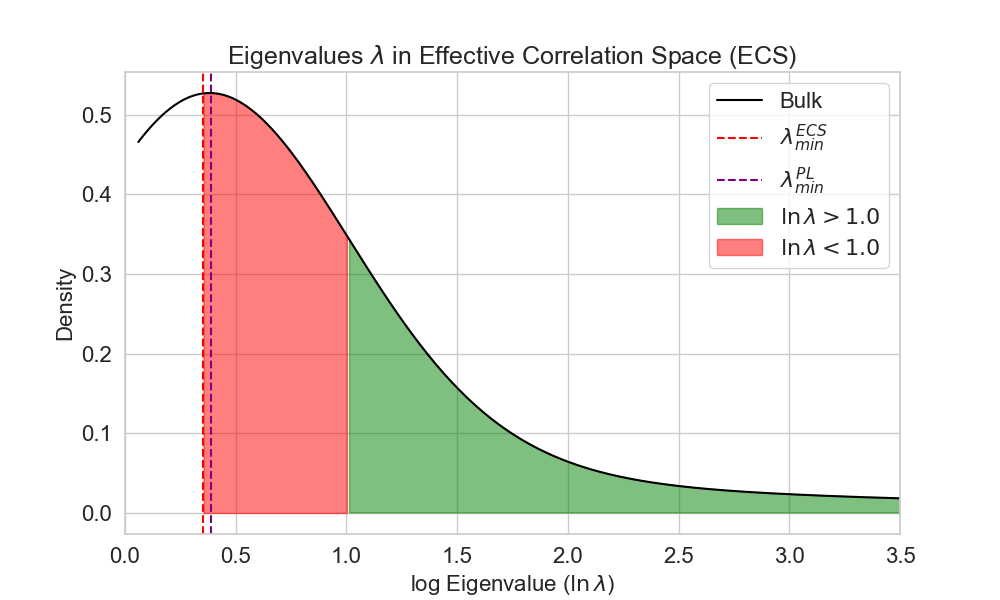
\includegraphics[width=10cm]{./img/ECS_space.png}
  \caption{The image depicts a typical
    \EmpiricalSpectralDensity (ESD) of a layer correlation matrix $\XMAT$, with \WW Power-Law (PL) exponent
    $\alpha=2.0$.%, normalized such that $\Trace{\XMAT}=\Vert\WMAT\Vert^{2}_{F}=N$.
    The green and red shaded regions depict
    eigenvalues $\lambda$ in the \EffectiveCorrelationSpace (\ECS) of $\XECS$, defined by $\lambda>\lambda_{min}^{ECS}$.
    The x-axis displays the eigenvalues on the log scale, $\ln\lambda$.
    The vertical red line is at the start of the PL tail  $(\lambda_{min}^{PL})$.
    The purple, vertical line is at the start of the~\ECS tail  $(\lambda_{min}^{ECS})$.
    The green shaded region depicts those eigenvalues where $\ln\lambda>1.0$,
    whereas the red shaded region depicts those eigenvalues where $\ln\lambda<1.0$.
    The~\ECS is defined such that the volume-preserving~\TRACELOG condition is best satisfied, i.e $\sum\ln\lambda= 0$ for $\lambda\ge\lambda_{min}^{ECS}$.
    }
  \end{center}
  \label{fig:ECS_space}
\end{figure}

Because the \Teacher ESD is most likely MHT and PL, 
if we choose $\lambda_{min}^{ECS}$ too small, and the tail extends too far into the bulk region of the ESD,
then for all practical purposes $\Det{\XECS}\ll 1$.
On the other hand, if we choose $\lambda_{min}^{ECS}$ too large,
then we only capture very large eigenvalues, and for all practical purposes $\Det{\XECS} \gg 1$.
Therefore, if we set the scale of $\XECS$ appropriately, we can choose a $\lambda_{min}^{ECS}$ such that $\Det{\XECS}=1$.
In this case, by choosing $\LambdaECSmin$ appropriately, we can estimate the expected value of
$\langle\Det{\AMATM}\rangle$  with an empirical point estimate over the \Teacher Correlation matrix, which is unity.
\begin{equation}
\label{eqn:detX}
\vert\det\XECS\vert \simeq 1 ; \quad \Trace{ \ln\XECS } = \ln\vert\det\XECS\vert \simeq 0  .
\end{equation} 

This expression can now be used in a practical calculation to define a low-rank subspace that both allows us to evaluate the HCIZ integral,
and to identify, in principle, generalizing components of the layer.
We also refer to \EQN~\ref{eqn:detX} as the \TRACELOG condition, which is technically its empirical form.
\michaeladdressed{Note by abuse of terminology.}
For example, Figure~\ref{fig:ECS_space} depicts the eigenvalues in the~\ECS for a \Typical ESD with PL $\alpha=2.0$..
Notice that the start of the PL tail, $(\lambda_{min}^{PL})$, is very close to the start of the~\ECS tail. $(\LambdaECSmin)$,
i.e. $\Delta \lambda_{min}:=\LambdaECSmin-\LambdaPLmin\approx 0$.
Also, notice that while there are many large eigenvalues, $\ln\lambda>1.0$, there are numerous small eigenvalues as well,
$\ln\lambda<1.0$, such that the $\sum\ln\lambda\approx 0$ for $\lambda\ge\lambda_{min}^{ECS}$. In other words, the red and green shaded areas have the same measure.
Additional plots like Figure~\ref{fig:ECS_space}, generated with \WW,  can be found in Section~\ref{sxn:empirical},
in Figure~\ref{fig:mlp3-detx-gap}
as well as plots of $\Delta \lambda_{min}$ vs. the \WW PL $\alpha$ for several real-world examples,
in Figures~\ref{fig:CV_ESD_trends} and ~\ref{fig:LLM_ESD_trends}.

